\section{Beschreibung des User Interface Konzepts}

[Detaillierte Beschreibung des Gesamtkonzepts: Wie wird das Interaktionsverhalten abgebildet? Wieso wurde diese Lösung gewählt? Wie wurden die Personas und Szenarios in der Konzeptausarbeitung berücksichtigt? Welche besonderen Prinzipien wurden bei der Realisierung beachtet?

Darstellung anhand der Abbildungen aller erstellten Wireframes oder Mockups und ggf. der Interaktionsabläufe als Flussdiagramm inkl. Beschreibung bzw. Erläuterung der dahinter stehenden Überlegungen in den folgenden Unterkapiteln. Der Zusammenhang der einzelnen Bildschirmmasken und Interaktionsfluss durch das Programm soll klar hervorgehen.]

\subsection{Desktop Web Interface}

\subsubsection{Navigation} \label{subsubsection:navigation}

% TODO: Inline figure

Die Navigationsleiste wird auf jedem Screen entlang der linken Bildschirmkante
angezeigt. Sie stellt eine Navigationshierarchie dar, die vom Benutzer geklickt
werden kann. Das aktuelle Element wird nach Applikationskonvention schwarz
dargestellt, andere Seiten dunkelgrau.  Momentan ist die Navigation relativ
spärlich besetzt, sie bietet aber reichlich Platz für eventuelle Erweiterungen
der Applikation.

\subsubsection{Aktuelles Monat} \label{subsubsection:aktuelles_monat}

% TODO: Inline figure

Ähnlich zur Navigationsleiste wird auf jedem Screen unten entlang der linken
Bildschirmkante eine kurze Zusammenfassung des aktuellen Monats dargestellt.
Der Benutzer erfährt auf einen Blick wichtige Kennzahlen wie zum Beispiel die
aktuell eingestellt Budgetgrenze, die bisherigen Monatsausgaben, das
verbleibende Budget, und Vergleiche mit dem Vormonat beziehungsweise dem
Durchschnitt aller Monate.

Wenn möglich werden diese Kennzahlen sowohl als Absolutbetrag sowie als
Prozentzahl dargestellt. Negative Abweichungen werden grün dargestellt (= man
hat im Vergleich dieses Monat gespart), positive mit roter Schriftfarbe.

\subsubsection{Übersicht}

\begin{figure}[htl]
\centering
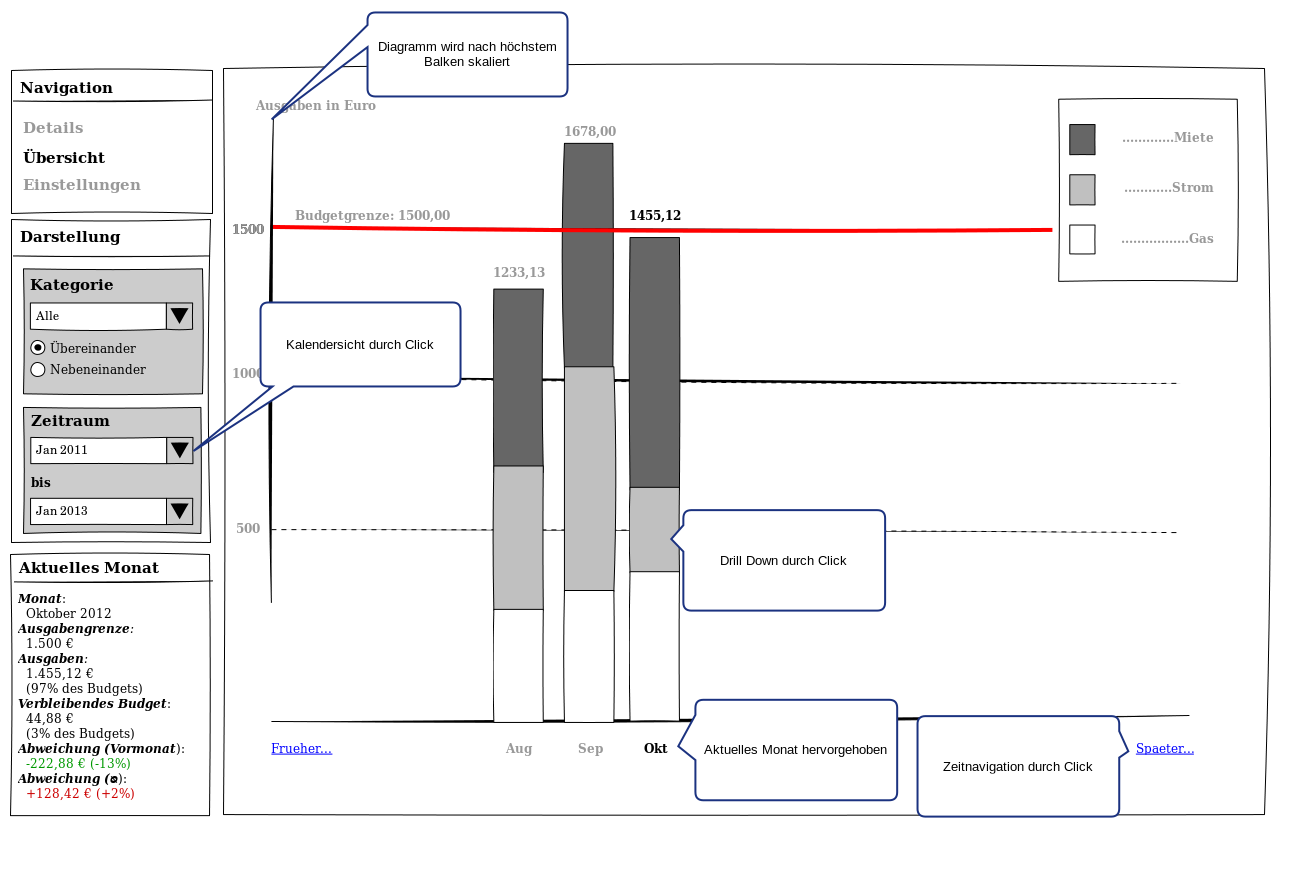
\includegraphics[width=\textwidth]{img/web_uebersicht}
\caption{Web \"Ubersicht}
\label{fig:web_uebersicht}
\end{figure}

In der Übersicht werden aggregierte Informationen zu den Finanzen dargestellt.
Dieser Screen kann durch einen Click auf 'Übersicht' innerhalb der
Navigationsleiste erreicht werden.

Auf der linken Seite des Bildschirms wird weiterhin (nach
Applikationskonvention) oben die Navigationsleiste (siehe Abschnitt
\ref{subsubsection:navigation}), und unten eine Zusammenfassung des aktuellen
Monats (siehe Abschnitt \ref{subsubsection:aktuelles_monat}) angezeigt.
Zusätzlich dazu werden nun Konfigurationsmöglichkeiten der
Übersichtsdarstellung angeboten, mithilfe dessen die Diagramme an
Benutzerpräferenzen angepasst werden können.

Es können die angezeigten Kategorien gefiltert werden; entweder werden alle
Kategorien angezeigt, oder man beschränkt sich auf eine bestimmte Kategorie.
Die Kategorieauswahl kann ebenfalls durch einen Click auf einen Balken
innerhalb des Diagramms getätigt werden. Die Darstellung der Kategorien kann
durch Radiobuttons entweder übereinander oder nebeneinander\footnote{Besonders
nützlich für Vergleiche zwischen Kategorien.} konfiguriert werden.  Wenn eine
bestimmte Kategorie ausgewählt ist werden die Radiobuttons ausgeblendet.

Es besteht außerdem die Möglichkeit zur Einstellung des angezeigten Zeitraums.
Durch einen Click auf eine der Zeitauswahlkomboboxen öffnet sich eine
Kalenderansicht. Der Zeitraum kann ebenfalls durch die Links 'Früher' und
'Später' im Diagramm geändert werden. Dadurch vergrößert sich der Zeitrahmen um
3 Monate in die jeweilige Richtung.

Das Diagramm selbst stellt Ausgaben (aggregiert nach Kategorie) pro Monat dar.
Die Diagrammskala wird jeweils nach dem höchsten Balken skaliert.  Die
eingestellte Budgetgrenze wird durch eine rote Linie dargestellt (falls sie
innerhalb das skalierte Diagramm fällt). Kategorien werden durch Farbkodierung
unterschieden, welche in der Legende aufgeschlüsselt ist. Achsen sind
selbstverständlich beschriftet; in der Monatsbeschriftung wird das aktuelle
Monat farblich hervorgehoben\footnote{Nach Applikationskonvention ist das
aktuelle Element schwarz, und alle anderen dunkelgrau}.


\subsection{Mobiles User Interface}
\subsection{Detailfragen}

\subsubsection{Frage 1}

\emph{Wie kann man Benutzer bei der Eingabe von Datensätzen unterstützen? Wie lassen sich Fehleingaben vermeiden? Wie werden diese Konzepte in Ihrem Prototypen realisiert?}

\vspace{2mm}


[Max. 250 Wörter, Wireframes zur Illustration]



\subsubsection{Frage 2}

\emph{Welche Informationen sind für Benutzer besonders wichtig und wie lässt sich deren Bedeutung im System repräsentieren? Welche Such-/Filter-/Sortier-Funktionen sind nützlich?}

\vspace{2mm}

Der Benutzer sollte auf einen Blick alle Ausgaben eines Monats sehen k\"onnen. Diese
werden auf der zentralen \"Ubersichtsseite chronologisch angeordnet dargestellt.

Ebenfalls sind einfache monatliche Zusammenfassungen wichtig; dazu wird in der
\"Ubersichtsseite am Ende jedes Monats eine Zusammenfassungszeile eingeblendet.
Die Zusammenfassung enth\"alt Informationen wie zum Beispiel die Summe aller monatlichen
Ausgaben, dessen Differenz zur festgelegten Budgetgrenze, und Vergleichswerte zu den Ausgaben
anderer Monate. Diese Zeile wird durch Schriftart und Hintergrundfarbe hervorgehoben.
Bei positiver Differenz (Grenze nicht \"uberschritten) ist die Differenz gr\"un dargestellt,
sonst rot.

Eintr\"age, die \"uber die Monatsgrenze hinausgehen werden durch rote Hintergrundfarbe
markiert.

Die Diagramme stellen vor allem Ausgaben pro Monat dar und sind als Balkendiagramme realisiert.
In diesem Zusammenhang ist nat\"urlich die Darstellung der monatlichen Obergrenze wichtig;
diese wird als Linie im Balkendiagramm eingezeichnet. Ebenfalls sind die Proportionen der Kategorien
von Interesse, deshalb wird ein Balken pro Kategorie eingef\"rbt.

Zur \"ubersichtlicheren Darstellung der Entwicklung von einzelnen Kategorien k\"onnen
diese auch in einem gefilterten Diagramm dargestellt werden (andere Kategorien werden
ausgeblendet).



\subsubsection{Frage 3}

\emph{Welche Möglichkeiten gibt es zur graphischen Aufbereitung der Daten (Grafiken, Kalender-Ansicht, etc.)? Wie werden diese Möglichkeiten in Ihrem Prototypen realisiert?}

\vspace{2mm}



[Max. 250 Wörter, Wireframes zur Illustration]



\subsubsection{Frage 4}

\emph{Wie lässt sich eine sinnvolle Aufgabenteilung zwischen Desktop-UI und mobiler UI erreichen? Welche Aufgaben haben bei der Verwendung zu Hause am Schreibtisch die höchste Priorität und welche Aufgaben haben bei der Verwendung am Smartphone die höchste Priorität? Welche Formen der graphischen Aufbereitung sind für den jeweiligen Anwendungskontext angemessen?}

\vspace{2mm}



[Max. 250 Wörter, Wireframes zur Illustration]
